\chapter{Overview and Preliminaries}
\label{chap:overview}

In this chapter, we present an overview of the whole thesis components, we present the system model, and some definitions.



\section{Overview}
In the end of this chapter, it should be clear how the different contributions are connected and how we materialize them in software systems. 


In a nutshell, as displayed in~Figure~\ref{fig:overview}, \system provides a distributed operating system for \gls{bft}-replicated services.
The system manages in its execution plane a set of nodes that can run \emph{unmodified replicas} (encapsulated in \glspl{vm} or containers). 
Each node must have a small \gls{ltu} that allows the activation and deactivation of replicas as demanded by the \system \emph{Controller}, in the control plane.
The controller decides which software should run at any given time by monitoring the existing vulnerabilities in the pool of replicas, aiming to minimize the risk of having several nodes being compromised by the same attack.

\begin{figure}[h]
\begin{center}
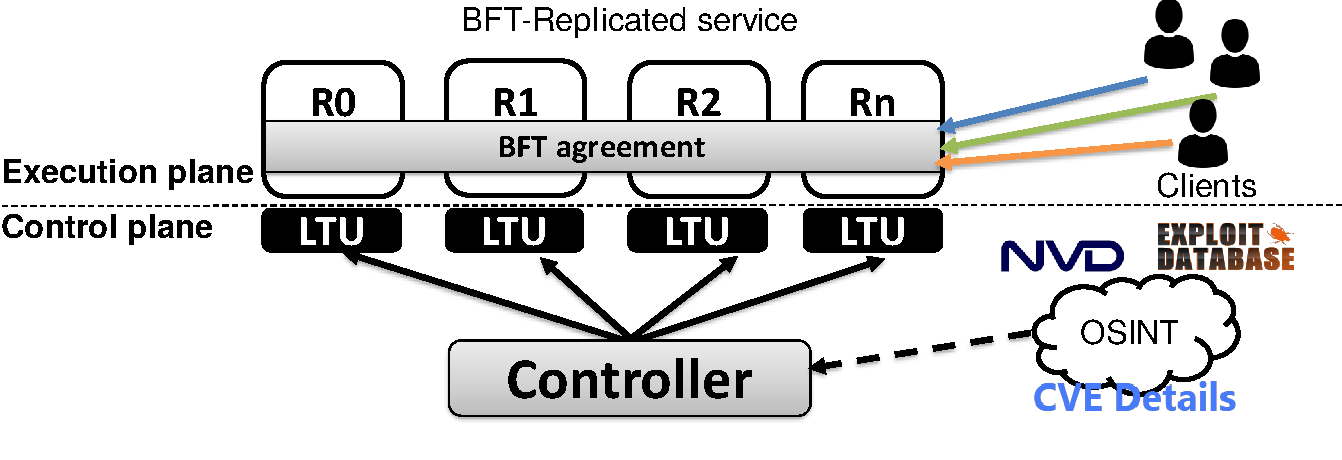
\includegraphics[width=0.7\columnwidth]{images/images/overview.pdf}
\vspace{-5mm}
\caption{\system overview.}
\label{fig:overview}
\end{center}
\end{figure}


\section{System Model}
\label{sec:systemmodel}

\system system model shares some similarity with previous works on the proactive recovery of \gls{bft} systems (e.g.,~\cite{Castro:2002,Platania:2014,Sousa:2010,Roeder:2010}).
More specifically, we consider a \emph{hybrid system model} composed of two planes with different properties and assumptions:

\begin{itemize}

\item \textbf{Execution Plane:} 
This plane is componsed of replica processes that can be subject to Byzantine failures.
Therefore, a Byzantine replica can try to mislead the other replicas or the clients.
These replicas communicate through an asynchronous network that can delay, drop or modify messages, just like most \gls{bft} system models~\cite{Castro:1999,Kotla:2010,Bessani:2014,Aublin:2015}.
This plane hosts $n$ replicas from which at most $f$ can be compromised at any given moment.
In this paper, we consider the typical scenario in which $n=3f+1$~\cite{Castro:2002,Kotla:2010,Aublin:2015}.  

\item \textbf{Control Plane:}  
For simplicity, we will address this component as a logical-centralized controller, which requires stronger assumptions. 
However, in Chapter~\ref{} we introduce \controller which requires weaker assumptions like the Execution Plane.

In this plane, we assume that each component can only fail by crashing. 
Each \emph{node} hosting processes contains a \gls{ltu}, and there is a logically-centralized controller to reconfigure the system, just like what has been used in several previous works on proactive recovery (e.g.,~\cite{Roeder:2010,Platania:2014,Sousa:2010}).
The failures of such components do not compromise the liveness and safety of the service as long as the control plane is recovered before $f$ replicas fail.


\end{itemize}

Besides the execution and control planes, we assume the existence of two types of external components: (1) clients of the replicated service, which can be subject to Byzantine failures; (2) \gls{osint} sources (e.g., \gls{nvd}, ExploitDB) that can not be subverted and controlled by the adversary.
In practice, this assumption lead us consider only well-established and authenticated data sources.
Dealing with untrusted sources is an active area of research in the threat intelligence community (e.g.,~\cite{Sabottke:2015,Liu:2015}), which we consider out of scope for this paper.


\section{Execution Plane}
\label{sec:executionplane}

The Execution Plane can accomodate any replicated system that already levareges on the existence of a controller node (e.g.,~\cite{Sousa:2010,Roeder:2010,Platania:2014,Garcia:2016}) or any \gls{bft} system that would benefit from the \system assistence (e.g.,~\cite{Sousa:2018}). 
However, a few requriements must be fulfilled, the Execution Plane is supported by virtulization therefore the \gls{bft} must run in a \gls{vm}.
Additionally, the \gls{bft} library must provide replicas configuration in order to allow replicas' replacement.
In this thesis we evaluate \system with three instances of differente Execution Planes: \gls{bft} ordering for Hyperledger Fabric, a \gls{kvs}, and \sieveq.
The latter, is one of the contributions of the thesis (see Chapter~\ref{chap:sieveq} and Chapter~\ref{chap:sieveqevaluation}, therefore detail its description.


\sieveq provides a message queue abstraction for critical services, applying various filtering rules to determine if messages are allowed to go through.
\sieveq is not a conventional firewall and we do not claim that it should replace existing firewalls in all deployment scenarios.
We are focusing on service- or information-critical systems that require a high-level of protection, and therefore, justify the implementation of advanced replication mechanisms.
The system we propose is able to deliver messages while guaranteeing authenticity, integrity, and availability.
As a consequence, and in contrast to conventional firewalls, we lose transparency on senders and receivers, since they are aware of the \sieveq's end-points.
The rest of the section explains how we address some of the mentioned issues and introduces the main design choices and the architecture of \sieveq.




Typical resilient firewall designs are based on primary-backup replication, and consequently, they are able to tolerate only crash failures.
Therefore, more elaborated failure modes may allow an adversary to penetrate into the protected network.


Some organizations deal with crashes (or \gls{dos} attacks) by resorting to several firewalls to support multiple entry points. 
This solution is helpful to address some (accidental) failures, but is incapable of dealing with an intrusion in a firewall.
In this case, the adversary gains access to the internal network, enabling an escalation of the attack, which at that stage can only be stopped if other protection mechanisms are in place.


Different fault tolerance mechanisms are employed at the two stages. 
Pre-filtering is implemented by a dynamic group of nodes named \presieves. 
\Presieves can be the target of various kinds of attacks and eventually may be intruded because they face the external network. Therefore, we take the conservative approach of assuming that \presieves can fail in an arbitrary (or Byzantine) way, meaning that they may crash or start to act maliciously.
When a failed \presieve is detected, it is simply replaced by a new one that is clean from errors.
Since \sieveq needs to support different message loads, e.g., due to additional senders, \presieves can be created dynamically to amplify the aggregated processing capabilities (within the constraints of the hardware).
The filtering stage is performed by a group of \repsieve components, which execute as a replicated state machine~\cite{Schneider:1990}.
\Repsieves may also fail in an arbitrary way, and therefore, we employ an intrusion-tolerant replication protocol that ensures correct operation in the presence of Byzantine faults.

Our solution was guided by the following design principles:

\begin{itemize}

\item \emph{Application-level filtering}: support sophisticated firewall filtering rules that take advantage of application knowledge. \sieveq implements this sort of rules by maintaining state about the existing flows, and this state has to be consistently replicated using a \gls{bft} protocol.

\item \emph{Performance}: address the most probable attack scenarios with highly efficient approaches, and as early as possible in the filtering stages; Reduce communication costs with external senders, as these messages may have to travel over high latency links (e.g., do not require message multicasts).	

\item \emph{Resilience}: tolerate a broad range of failure scenarios, including malicious external/internal attackers, compromised authenticated senders, and intrusions in a subset of the \sieveq components; Prevent malicious external traffic from reaching the internal network by requiring explicit message authentication.

\end{itemize}



\section{Control Plane}
\label{sec:controlplane}

\system is the first control plane that automatically changes the attack surface of a \gls{bft} system in a dependable way.
\system continuously collects security data from \gls{osint} feeds on the internet to build a knowledge base about the possible vulnerabilities, exploits, and patches related to the systems of interest.
This data is used to create clusters of similar vulnerabilities, which potentially can be affected by (variations of) the same exploit.
These clusters and other collected attributes are used to analyze the risk of the \gls{bft} system becoming compromised. % due to common vulnerabilities.
Once the risk increases, \system replaces the potentially vulnerable replica by another one, trying to maximize the failure independence. % of the replicated service.
Then, the replaced node is put on quarantine and updated with the available patches, to be re-used later.
These mechanisms were implemented to be fully automated, removing the human from the loop.

The current implementation of \system manages 17 \gls{os} versions, supporting the \gls{bft} replication of a set of representative applications.
The replicas run in \glspl{vm}, allowing provisioning mechanisms to configure them. 
We conducted two sets of experiments, one demonstrates that \system risk management can prevent a group of replicas from sharing vulnerabilities over time; the other, reveals the potential negative impact that virtualization and diversity can have on performance. 
However, we also show that if naive configurations are avoided, \gls{bft} applications in diverse configurations can actually perform close to our homogeneous bare metal setup.

\subsection{BFT-Control Plane}
\note{add details later}

\section{Diversity of Replicas}
\label{sec:diversityofreplicas}
\note{citar survey \cite{Baudry:2015}}
%BFT-replicated services running on \system are composed by $n$ replicas.
For our purposes, each \replica is composed of a stack of software, including an OS (kernel plus other software contained in an \gls{os} distribution), execution support (e.g., \gls{jvm}, \gls{dbms}), a \gls{bft} library, and the service that is provided by the system.
%(see Figure~\ref{fig:arch1}).
The set of $n$ replicas is called a \configuration.

It is possible to improve the \replicas fault independence by resorting to different \gls{ots} components in the software stack~\cite{Deswarte:1998}. 
For example, it has been shown that using distinct \glspl{os}~\cite{Garcia:2014}, filesystems~\cite{Rodrigues:2001,Bairavasundaram:2009}, and databases~\cite{Gashi:2007}, can yield important benefits in terms of fault independence. In addition, automatic techniques could enhance diversity, like randomization/obfuscation of \glspl{os}~\cite{Roeder:2010} and applications~\cite{King:2016}.

Although \system can exploit automatic techniques, in this paper we center our attention on diverse \gls{ots} components. 
In particular, \system monitors the disclosed vulnerabilities of all elements of the software stacks of the replicas to assess which of them may contain common vulnerabilities.  

However, in the experimental evaluation, we focus on the diversity of OSes (not only the kernel, but the whole product) for three fundamental reasons: (1) by far, most of the replica’s code is the \gls{os}; (2) such size and importance, make \glspl{os} a valuable target, with new vulnerabilities and exploits being discovered every day; and (3) there are many options of OSes that can be used.
The two last factors are particularly important to enrich the validity of our analysis.

Moreover, we do not explicitly consider the diversity of the \gls{bft} library (i.e., the protocol implementation) or the service code implemented on top of it.
Four facts justify this decision: (1) N-version programming is too costly for this~\cite{Avizienis:1977}; (2) there have been some works showing that such protocol implementations can be generated from formally verified specifications~\cite{Hawblitzel:2015,Rahli:2018}; (3) the relatively small size of such components (e.g., a key-value store on top of BFT-SMaRt has less than 15k lines of code~\cite{Bessani:2014}) make them relatively simple to test and assess with some confidence~\cite{Martins:2013,Lee:2014};  and (4) there are no reported vulnerabilities about these system to support our study.
Notice that, although we do not explicitly consider the diversity of \gls{bft} libraries, nothing prevents \system from monitoring them (when several alternatives become available). 
Additionally, as a pragmatic approach, we could employ automatic diversity techniques in this layer~\cite{Platania:2014,Roeder:2010}.


